\documentclass[tikz,border=10pt]{standalone}
\usetikzlibrary{angles,quotes,calc}
\begin{document}
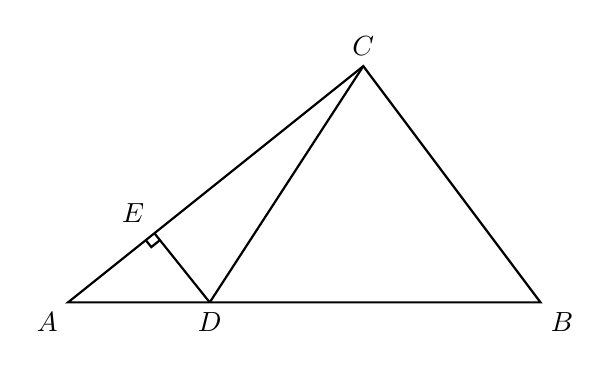
\begin{tikzpicture}[scale=1.5, thick]    
% 1. 定义顶点坐标    
\coordinate (A) at (0,0);    
\coordinate (B) at (4,0);    
\coordinate (C) at (2.5,2);        
% 2. 定义点 D 在 AB 上 (比例可调整)    
\coordinate (D) at (1.2,0);        
% 3. 计算点 E: DE 垂直于 AC    
% 使用投影计算点 E (D 在直线 AC 上的投影)    
\coordinate (E) at ($(A)!(D)!(C)$);        
% 4. 绘制三角形 ABC    
\draw (A) -- (B) -- (C) -- cycle;        
% 5. 绘制线段 CD 和 DE    
\draw (C) -- (D);    
\draw (D) -- (E);        
% 6. 标注顶点标签    
\node[below left] at (A) {$A$};    
\node[below right] at (B) {$B$};    
\node[above] at (C) {$C$};    
\node[below] at (D) {$D$};    
\node[above left] at (E) {$E$};        
% 7. 绘制直角标记 (使用 tkz-euclide 或原生写法)    
\draw ($(E)!0.1!(D)$) -- ($(E)!0.1!(D) + (E)!0.1!(A) - (E)$) -- ($(E)!0.1!(A)$);

\end{tikzpicture}
\end{document}